\chapter{Methodology}
\section{Introduction}
Deep learning is a multidisciplinary field ranging from linear algebra, calculus and probability theory. With major advancement made in compute processing power; deep learning is commonly used in the industry now.
\section{Linear Algebra}
We introduce briefly the realm of linear algebra to get a better understanding of more complex concepts in neural networks. The focus is set on mainly the properties useful in deep learning. \\
Linear algebra is the study of linear equations of the form:
\begin{equation}
    x_1a_1 + \dots + x_na_n = b
\end{equation}
or as a linear map defined by the following:
\begin{equation}
    (x_1, \dots, x_n) \mapsto (a_1 x_1 + \dots + a_n x_n) \label{eq:2.11}
\end{equation}
and their representation, manipulation and operation using vectors and matrices within a set of predefined axioms. 
\subsection{Vectors}
A vector is quantity that has both a magnitude and direction. It can be represented by an ordered set of numbers or graphically using an arrow.
Consider the vector \textbf{u} in $\mathbb{R}^2$ given by:
\begin{align}
    \textbf{u} &= \begin{bmatrix}
           u_1 \\
           u_2 \\
         \end{bmatrix}
  \end{align}
The vector can be expressed graphically as shown below.
\begin{center}
    *Image Placeholder vector in $R^2$*    
\end{center}

\noindent The length of the arrow is an indication of the magnitude of a vector and its orientation given by the direction in which the arrow is pointing. The magnitude of the above vector can be computed as such:
\begin{align}
    ||\textbf{u}|| = \sqrt{u_1^2+u_2^2}
\end{align}

\noindent The direction of the vector with respect to the $x$-axis is given by: 
\begin{align}
    \theta = \tan^{-1}\left(\dfrac{u_2}{u_1}\right)
\end{align}
A vector space is a set of vectors which satisfy the following axioms:
\begin{center}
    *Placeholder - Table of Axioms for Vector Space*    
\end{center}
\noindent\textbf{Geometry representation of addition and subtraction of vectors in $\mathbb{R}^2$}
Vector addition and subtraction is performed componentwise along each element of two vectors. Consider the two vectors $\textbf{a}$ and $\textbf{b}$ where:
\begin{align}
    \textbf{u} = \begin{bmatrix}
        u_1 \\
        u_2 \\
      \end{bmatrix},
      \textbf{v} = \begin{bmatrix}
        v_1 \\
        v_2 \\
      \end{bmatrix}
\end{align}
\noindent\textbf{Addition} \\
The addition of vector $\textbf{u}$ and $\textbf{v}$ is given by:
\begin{align}
    \textbf{u} + \textbf{v} =
      \begin{bmatrix}
        u_1 + v_1 \\
        u_2 + v_2 \\
      \end{bmatrix}
      \label{eq:addition_vectors}
\end{align}
The geometrical effect of adding $\textbf{u}$ and $\textbf{v}$ together is shown below.
\begin{center}
    *Image Placeholder vector addition in $R^2$*    
\end{center}
We can observe from (image ref) above that adding $\textbf{u}$ to $\textbf{v}$ has the effect of rotating $\textbf{u}$ towards $\textbf{v}$.

\noindent\textbf{Subtraction} \\
The subtraction of vector $\textbf{v}$ from $\textbf{u}$ is given by:
\begin{align}
    \textbf{u} - \textbf{v} =
      \begin{bmatrix}
        u_1 - v_1 \\
        u_2 - v_2 \\
      \end{bmatrix}
      \label{eq:subtraction_vectors}
\end{align}
\begin{center}
    *Image Placeholder vector subtraction in $R^2$*    
\end{center}
We can observe from (image ref) above that subtracting $\textbf{v}$ from $\textbf{u}$ has the effect of rotating $\textbf{u}$ in the opposite direction of $\textbf{v}$.\\
\vspace{1mm}
\noindent The effect of rotating two vectors though addition and subtraction are useful properties utilized in deep learning.
\subsubsection{Inner Product}
\noindent The inner product or dot product of: 
\begin{align}
    \textbf{u} = \begin{bmatrix}
        u_1 \\
        u_2 \\
      \end{bmatrix},
      \textbf{v} = \begin{bmatrix}
        v_1 \\
        v_2 \\
      \end{bmatrix}
\end{align}
is given by $\textbf{u}.\textbf{v}$
\begin{align}
  \textbf{u.v} &= u_1 v_1 + u_2 v_2 \\
  &= ||\textbf{u}|| \, ||\textbf{v}||\cos \theta
  \label{eq:cosine_rule_dot_product}
\end{align}
where $\theta$ is the angle between vectors \textbf{u} and \textbf{v}.
\begin{center}
  *Image Placeholder inner product in $R^2$*    
\end{center}
The dot product of $\textbf{u.v}$ equals \textbf{v.u}. The order does not make a difference.
\subsection{Matrices}
\noindent A matrix is an $m \times n$ array of numbers, where $m$ is the number of rows and $n$ is the number of columns; the matrix is said to be of dimension $(m \times n)$.
\begin{align}
  \textbf{A} = 
  \begin{bmatrix}
    a_{11} & a_{12} & \dots & a_{1n} \\
    a_{21} & a_{22} & \dots & a_{2n} \\
    \vdots & \vdots & \ddots & \vdots \\
    a_{m1} & a_{m_2} & \dots & a_{mn}
  \end{bmatrix}
\end{align}
Similar to vectors, there are a couple of matrix operations that can be done under certain condition. \\
\noindent \textbf{Matrix Operations} \\ 
\noindent \textbf{Matrix Addition} \\
The sum of two matrices $\textbf{A}$ and $\textbf{B}$ is given by the element wise sum of the elements provided that they both have the same dimension. 
\\ Consider two matrices \textbf{A} and \textbf{B}:
\begin{align}
  \textbf{A} =
  \begin{bmatrix}
    a_{11} & a_{12} \\
    a_{21} & a_{22}
  \end{bmatrix} \, \, \, 
  \textbf{B} =
  \begin{bmatrix}
    b_{11} & b_{12} \\
    b_{21} & b_{22}
  \end{bmatrix}
\end{align}
 the sum \textbf{A + B} is given by
\begin{align}
  \textbf{A} + \textbf{B} = \begin{bmatrix}
    a_{11} + b_{11} & a_{12} + b_{12} \\
    a_{21} + b_{21} & a_{22} + b_{22}
  \end{bmatrix}
\end{align}\\
\noindent \textbf{Scalar Matrix Multiplication} \\
The product $\alpha\textbf{A}$, where $\alpha \in \mathbb{R}$ and $\textbf{A}$ is a matrix, is calculated by multiplying every entry of $\textbf{A}$ by $\alpha$. \\
Consider  a matrix \textbf{A} and constant $\alpha$:
\begin{align}
  \begin{bmatrix}
    a_{11} & a_{12} \\
    a_{21} & a_{22}
  \end{bmatrix}
\end{align}
the scalar multiplication $\alpha \textbf{A}$ is given by
\begin{align}
  \alpha \textbf{A} = 
  \alpha \begin{bmatrix}
    a_{11} & a_{12} \\
    a_{21} & a_{22}
  \end{bmatrix}
  = \begin{bmatrix}
    \alpha a_{11} & \alpha a_{12} \\
    \alpha a_{21} & \alpha a_{22}
  \end{bmatrix}
\end{align} \\
\noindent \textbf{Matrix Transpose} \\
\noindent The transpose of a $(m \times n)$ matrix $\textbf{A}$ is calculated by swapping the rows into columns or the columns into rows. This operation result in a $(n \times m)$ denoted as $\textbf{A}^T$. \\
Consider  a matrix \textbf{A}, the transpose is given by $\textbf{A}^T$:
\begin{align}
  \textbf{A} = \begin{bmatrix}
    a_{11} & a_{12} \\
    a_{21} & a_{22}
  \end{bmatrix} \, \, \, 
  \textbf{A}^T = \begin{bmatrix}
    a_{11} & a_{21} \\
    a_{12} & a_{22}
  \end{bmatrix}
\end{align}
\noindent \textbf{Matrix Multiplication} \\
The multiplication operation between two matrices is only defined is the number of columns of the left matrix is the same as the number of rows in the right matrix. If \textbf{A} is a $(m \times n)$ matrix and \textbf{B} is a $(n \times p)$ matrix, then their product \textbf{AB} is the $(m \times n)$ matrix whose entries are given by inner product of the corresponding row of \textbf{A} and the corresponding column of \textbf{B}.\\
Consider two matrices \textbf{A} and \textbf{B}:
\begin{align}
  \textbf{A} =
  \begin{bmatrix}
    a_{11} & a_{12} & a_{13} \\
    a_{21} & a_{22} & a_{23}
  \end{bmatrix} \, \, \, 
  \textbf{B} =
  \begin{bmatrix}
    b_{11} & b_{12} \\
    b_{21} & b_{22} \\
    b_{31} & b_{32}
  \end{bmatrix}
\end{align}
 the matrix multiplication is given by \textbf{AB}
\begin{align}
  \textbf{A}\textbf{B} &= \begin{bmatrix}
    a_{11} & a_{12} & a_{13} \\
    a_{21} & a_{22} & a_{23}
  \end{bmatrix} \begin{bmatrix}
    b_{11} & b_{12} \\
    b_{21} & b_{22} \\
    b_{31} & b_{32}
  \end{bmatrix} \\
  &= \begin{bmatrix}
    a_{11}b_{11} + a_{12}b_{21} + a_{13}b_{31} &  a_{11}b_{12} + a_{12}b_{22} + a_{13}b_{32} \\
    a_{21}b_{11} + a_{22}b_{21} + a_{23}b_{31} &  a_{21}b_{12} + a_{22}b_{22} + a_{23}b_{32}
  \end{bmatrix}
\end{align}
\subsubsection{Outer Product}
\noindent The outer product of two vectors $\textbf{u}$ and $\textbf{v}$: 
\begin{align}
    \textbf{u} = \begin{bmatrix}
        u_1 \\
        u_2 \\
      \end{bmatrix} \, \, \, 
      \textbf{v} = \begin{bmatrix}
        v_1 \\
        v_2 \\
      \end{bmatrix}
\end{align}
is given by $\textbf{u}\otimes\textbf{v}$
\begin{align}
  \textbf{u}\otimes\textbf{v} = \begin{bmatrix}
    u_1v_1 & u_1v_2 \\
    u_2v_1 & u_2v_2
  \end{bmatrix}
\end{align}
The outer product of $\textbf{u}\otimes\textbf{v}$ is not equal to $\textbf{v}\otimes\textbf{u}$; the order does matter. However, the transpose of latter outer product are the same:
\begin{align}
  \textbf{u}\otimes\textbf{v} = (\textbf{v}\otimes\textbf{u})^T
\end{align}
\section{Differential calculus}
Differential calculus is the study of the definition, properties, and applications the derivative of a function. The process of finding the derivative is called differentiation. It is the also referred to as the study of rate of change and slopes of curves. In optimization and deep learning, major concepts of differential calculus are used.
\subsection{Derivatives}
Derivatives are important concept for understanding deep learning. The derivative of a function at a particular point is the rate of change of the output of the function with respect to the input at that point. It is also an indication of the slope of the function at a particular point.\\
The mathematical definition of the derivative of a function $f = f(x)$ at a point $a$ is given by
\begin{align}
  f^{'}(a) &= \frac{df}{d x}(a) \\ 
  &= \lim_{\Delta \rightarrow 0} \frac{f(a+\Delta) - f(a-\Delta)}{2 \times \Delta}
\end{align}
\begin{center}
  *Image Placeholder derivative of a function $f$ at $a$ in $\mathbb{R}^2$  and $\mathbb{R}^3$*    
\end{center}
Since the derivative of a function is an indication of the slope of a function; we can deduce that a minimum or maximum point exists when the derivative is equal to $0$ (may also be indication of an inflection point).

\vspace{5mm}
\noindent \textbf{Derivative of Multivariate Functions}
\subsection{Directional Derivatives}
\subsection{Chain Rule}
 The chain rule is a concept in calculus to help us understand and calculate the derivative for composite functions which can be made up of two or more functions chained together. \\
Suppose that we have two function $f(x)$ and $g(x)$ which are both differentiable and define the composite function $h(x) = f(g(x))$ then the derivative of $h^{'}(x)$ is given by
\begin{align}
  h^{'}(x) &= \dfrac{dh}{dx} \\
  &= f^{'}(g(x))g^{'}(x)
\end{align}
Consider that we  have $y=f(u)$ and $u=g(x)$, a different definition of the composite function $y=f(g(x))$, then the derivative of $y$ is,
\begin{align}
  h^{'}(x)  &= \dfrac{dh}{dx} \\
  &= \dfrac{dh}{du} \dfrac{du}{dx}
\end{align}
\subsection{Hessian}
\section{Optimization}
The optimization problem is a computational problem in which the objective is to find the best of all possible solutions. Deep neural networks is a form of an optimization problem to find the best possible set of weights in order to reduce the error in a network.

\noindent A generic form of an optimization problem is given by 
\begin{align}
  \begin{matrix}
    \underset{x}{\text{minimize/maximize}} &f(x) & \\
    \text{subject to} &g_i(x) \leq 0, \, \, & i=1,\dots,m \\
    &h_j(x) = 0, & j=1,\dots,p
  \end{matrix}
  \label{eq:optimization_problem}
\end{align} 
\noindent where \\
\indent $f: \mathbb{R}^n \rightarrow \mathbb{R}$ is the objective/loss function to be minimized,\\
\indent $g_i(x) \leq 0$ are called inequality constraints,\\
\indent $h_j(x) = 0$ are called equality constraints, and \\
\indent $m\geq0$ and $p\geq0$

\vspace{5mm}
\noindent If $m=p=0$, the problem is an unconstrained optimization problem.
\subsection{Optimization algorithms}
The solutions to the optimization problem are vital in modern machine learning and artificial intelligence algorithms, which includes weight optimization in deep learning. There are a number of popular optimization algorithm currently developed to solve the problem. Hence, choosing the right algorithm can be challenging as well.
\vspace{5mm}
\noindent We explore few of the gradient-based solution to the optimization below. Gradient-based methods are iterative methods that use the gradient information of the objective function during iterations.

\vspace{5mm}
\noindent\textbf{Newton's Method}\\
For minimizing $f(x)$, $x \in \mathbb{R}$, we need to solve $g(x) = f^{'}(x)=0$. Newton's iteration is given by 
\begin{align}
  x_{n+1} &= x_{n} - \dfrac{g(x_{}n)}{g^{'}(x_n)} \\
          &= x_{n} - \dfrac{f^{'}(x_{}n)}{f^{''}(x_n)}
\end{align}
For multivariate functions we need to minimize $f(\mathbf{x})$ over $\mathbf{x} \in \mathbb{R}^n$, that it
\begin{align}
  \begin{matrix}
    \underset{\mathbf{x}\in\mathbb{R}^n}{min} f(\mathbf{x}), & \,\,\, \mathbf{x} =(x_1,x_2,\dots,x_n)^T \in \mathbb{R}^n
  \end{matrix} 
\end{align}
The Newton's iteration for multivariate function is given by
\begin{align}
  \mathbf{x_{n+1}} = \mathbf{x_{n}} - H(\mathbf{x_n})^{-1}\nabla f(\mathbf{x_n})
\end{align}
where\\
\indent $H(\mathbf{x_n})$ is the Hessian matrix of $f(\mathbf{x})$\\
\noindent We can observe from (equation ref) that calculating the inverse of the Hessian matrix can be computationally very expensive for higher dimensions. Replacing $H(\mathbf{x_n})^{-1}$ by $\alpha \mathcal{I}$ where $\mathcal{I}$ is the identity matrix; we get the \textbf{method of steepest descent} given by
\begin{align}
  \mathbf{x_{n+1}} = \mathbf{x_{n}} - \alpha \textbf{I} \nabla f(\mathbf{x_n})
\end{align}
where $\alpha \in (0,1)$ 
\section{Deep Learning}
%\noindent - Short dive into deep learning and its advancement in recent years
%\noindent - Explanation of OR and XOR functions
Deep learning is part of Machine Learning which deals mainly with computers that can learn either on their own or supervised. The latter can solve problem in the industry ranging from computer vision (image), natural language processing (text), automatic speech recognition (audio), time-series prediction amongst others. Deep learning primarily uses the concept of artificial neural networks, which derivatives from how the human brain works, to solve complex linear and non-linear problem.\\
\indent We start by introducing how a simple perceptron works, and gradually increase the complexity of the network until we reach a deep neural network that can solve non-linear problems.
\subsection{Perceptron}
%- Explanation on neuron and short numeric exercise \\ 
%- Solving the XOR OR function using Perceptron
A perceptron is an analogy to the human neuron. It is a computational model that takes an input (scalar or vector) and learns to classify the latter between two classes (binary classifier). It consists of an input, a weighed sum and an activation function. \\ The mathematical definition a perceptron that maps its input $\textbf{x}$ to an output value $f(\textbf{x})$ using a step function as activation function is given by
\begin{align}
  f(\textbf{x}) =
  \begin{cases}
    1 & \text{if } \textbf{w.x} + b > 0 \\
    0 & \text{otherwise}
    \label{eq:perceptron_def}
  \end{cases}
\end{align}
\begin{figure}[h]
  \centering
  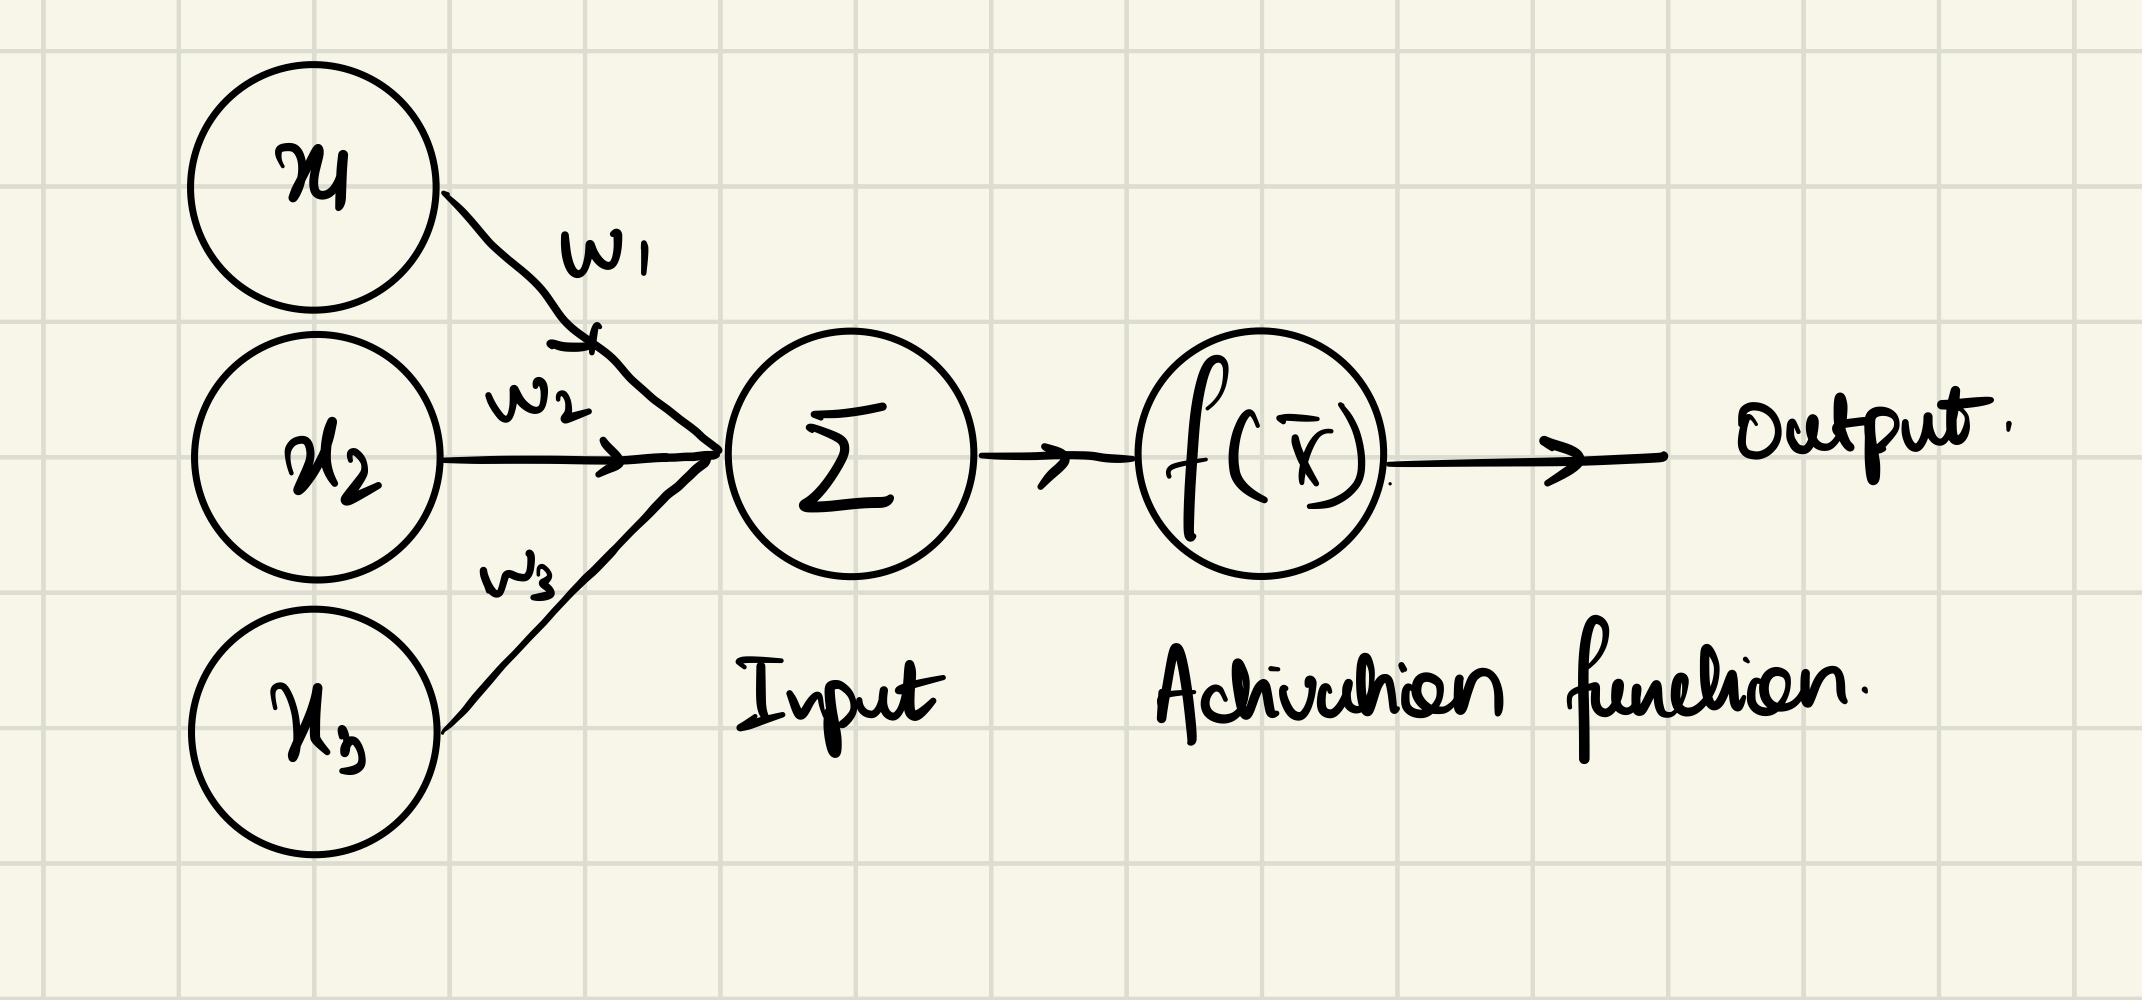
\includegraphics[scale=0.15]{CHAPTER_2/c2_fig_perceptron.jpeg}
  \caption{Perceptron graphical representation}
  \label{fig:perceptron}
\end{figure}\\
From the perceptron mathematical definition \refeq{eq:perceptron_def}, we can observe that the dot product is dependent on the angle between the weight vector (\textbf{w}) and the input vector (\textbf{x}). Using dot product (\refeq{eq:cosine_rule_dot_product}), addition (\refeq{eq:addition_vectors}) and subtraction (\refeq{eq:subtraction_vectors}) of vector property; we can define a learning rule for modifying the perceptron to learn how to classify a set of input.
\subsubsection{Perceptron Learning Rule}
\noindent Consider the two sets of point \textbf{A} and \textbf{B} 
\begin{align}
  \textbf{A} =
  \begin{Bmatrix}
    \begin{bmatrix}
      1 \\ 
      2
    \end{bmatrix}
  \end{Bmatrix}
   \, \, \, 
  \textbf{B} =
\begin{Bmatrix}
  \begin{bmatrix}
    -1 \\
    2
  \end{bmatrix},
  \begin{bmatrix}
    0 \\
    -1
  \end{bmatrix}
  \end{Bmatrix}
\end{align}
and fitting the perceptron function (\refeq{eq:perceptron_def}) to learn how to classify points in each respective set. Let set \textbf{A} and \textbf{B} be class 1 and 0 respectively.
\begin{figure}[h]
  \centering
  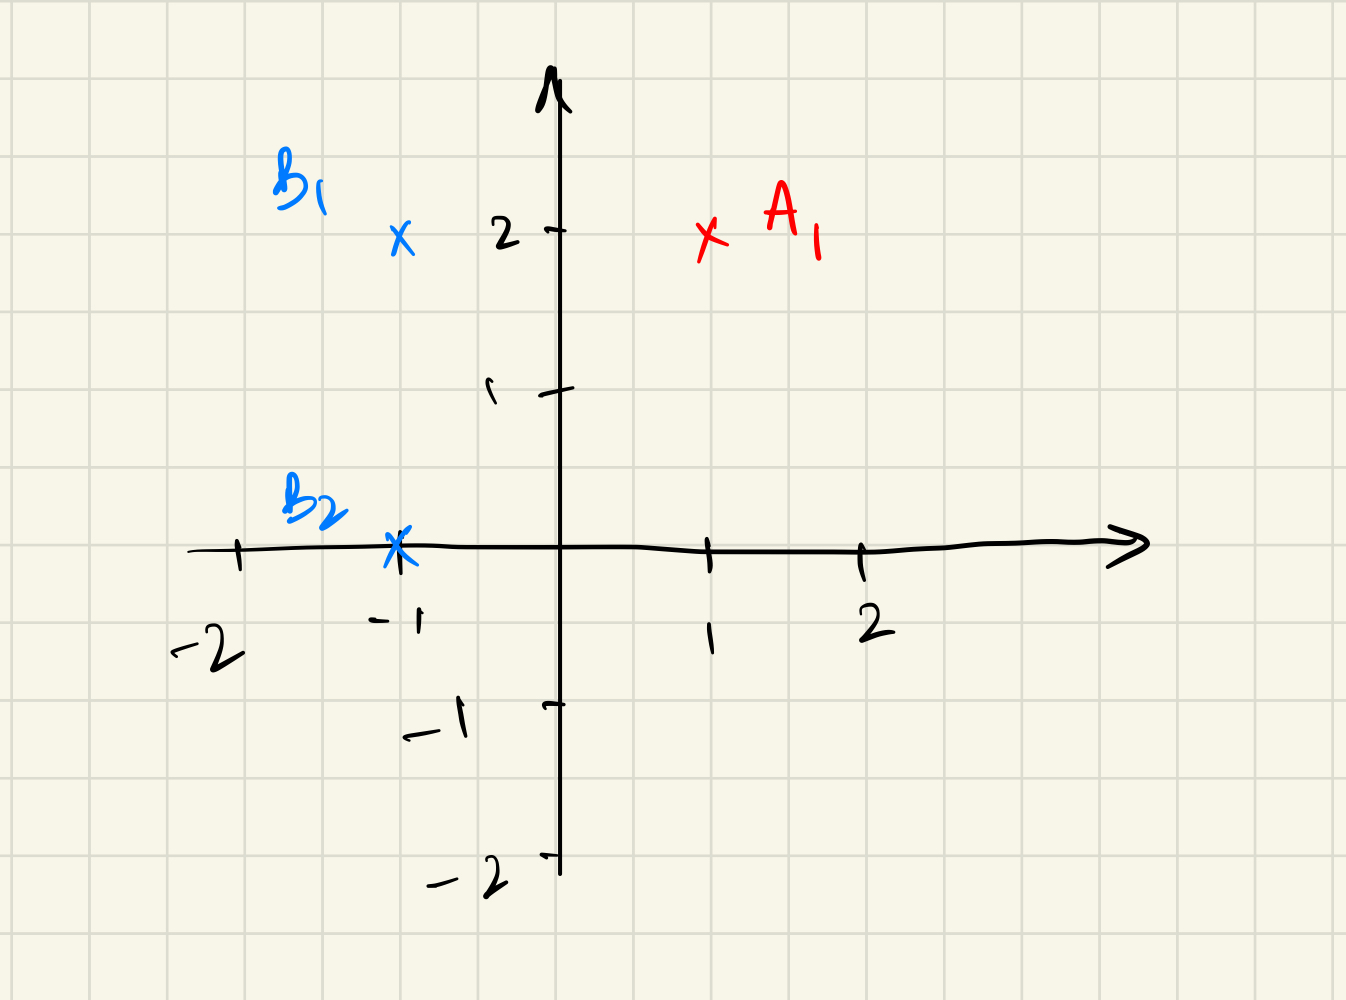
\includegraphics[scale=0.15]{CHAPTER_2/c2_fig_perceptron_example_1.jpeg}
  \caption{Caption}
  \label{fig:perceptron_example_1}
\end{figure}\\
From \ref{fig:perceptron_example_1}, we can separate the two classes by a single line. Consider the random separating line passing through the origin (this will set the value of b in (\refeq{eq:perceptron_def}) to 0).\\
\begin{figure}[!htbp]
  \centering
  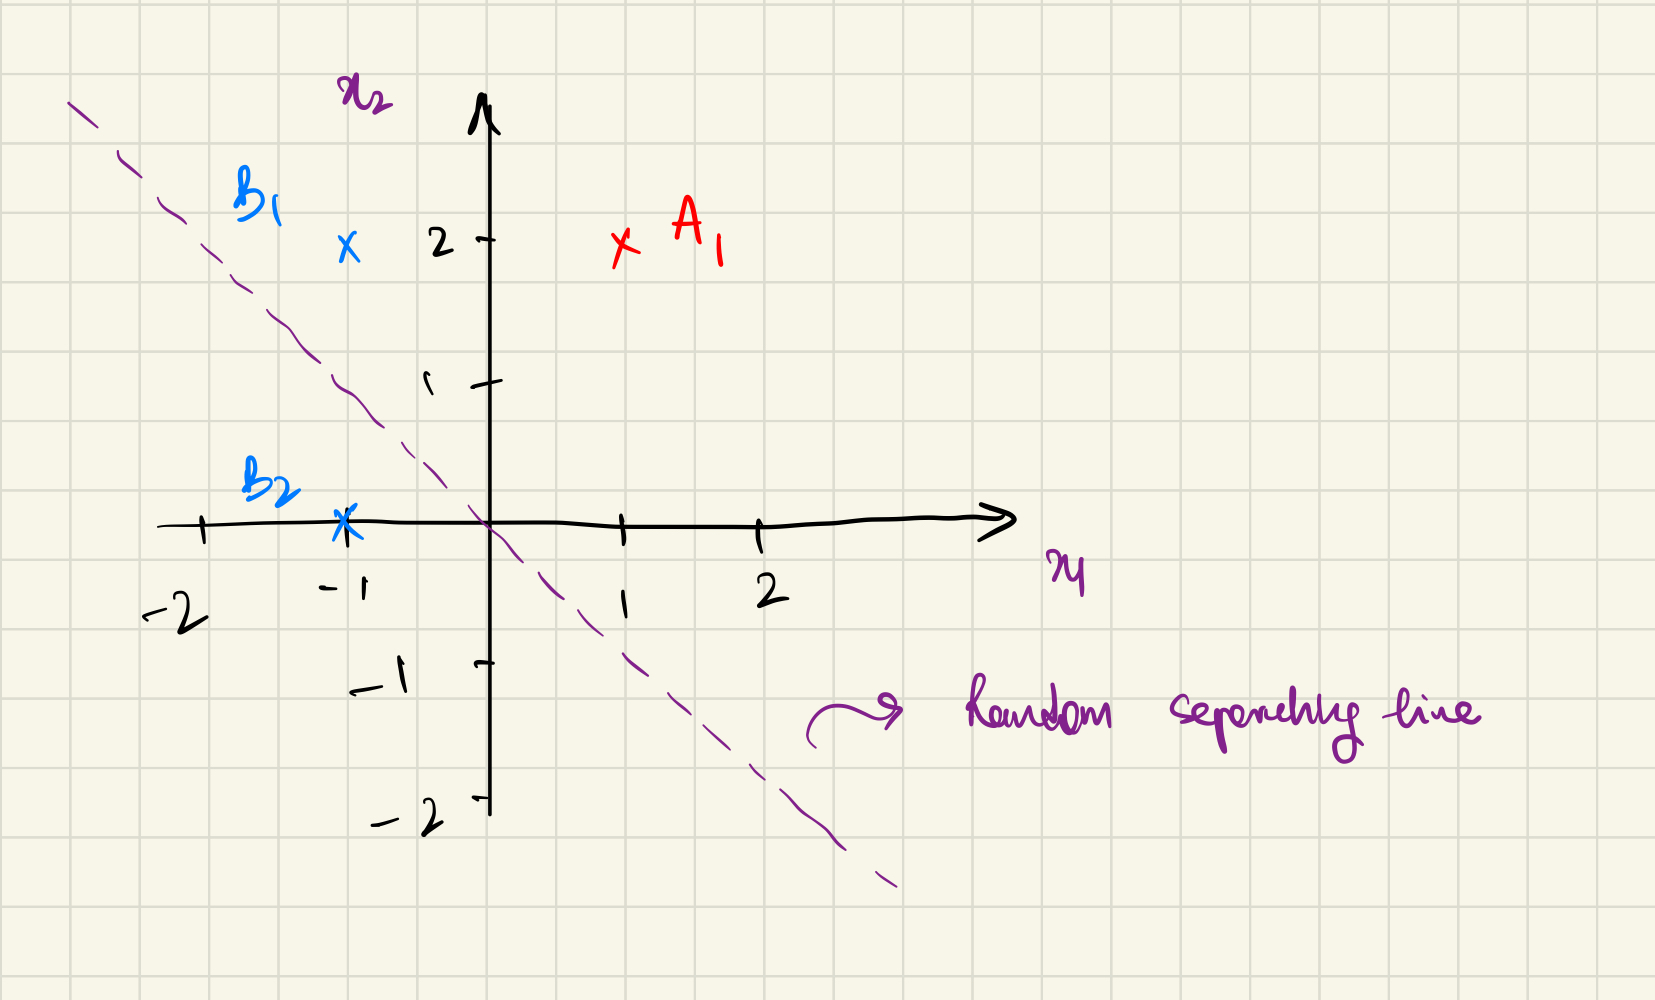
\includegraphics[scale=0.15]{CHAPTER_2/c2_fig_perceptron_example_2.jpeg}
  \caption{Caption}
  \label{fig:perceptron_example_2}
\end{figure}\\
The equation of the random line is given by
\begin{align}
  x_1 = - x_2
\end{align}
Comparing to the equation (\refeq{eq:perceptron_def}); we can deduce that 
\begin{align}
  \begin{matrix}
    w_1 = 1 & w_2 = 1
  \end{matrix}
\end{align}
Visually, we can already see that the separating line does not split the points properly. The computation of the binary classification using the random line is given by
\begin{align}
  f(A_1) &= f\begin{pmatrix}
    \begin{bmatrix}
      1\\
      1
    \end{bmatrix}.\begin{bmatrix}
      1 \\
      2
    \end{bmatrix}
  \end{pmatrix} = f(3) = 1 \\
  f(B_1) &= f\begin{pmatrix}
    \begin{bmatrix}
      1\\
      1
    \end{bmatrix}.\begin{bmatrix}
      -1 \\
      2
    \end{bmatrix}
  \end{pmatrix} = f(1) = 1 \\
  f(B_2) &= f\begin{pmatrix}
    \begin{bmatrix}
      1\\
      1
    \end{bmatrix}.\begin{bmatrix}
      -1 \\
      0
    \end{bmatrix}
  \end{pmatrix} = f(-1) = 0
\end{align}
The computation confirms the visual representation and groups $\textbf{A}_1$ and $\textbf{B}_1$ together. We can either alter the separating line (by moving the weight vector) with respect to $\textbf{A}_1$ and/or $\textbf{B}_1$.\vspace{50mm}
\begin{figure}[h]
  \centering
  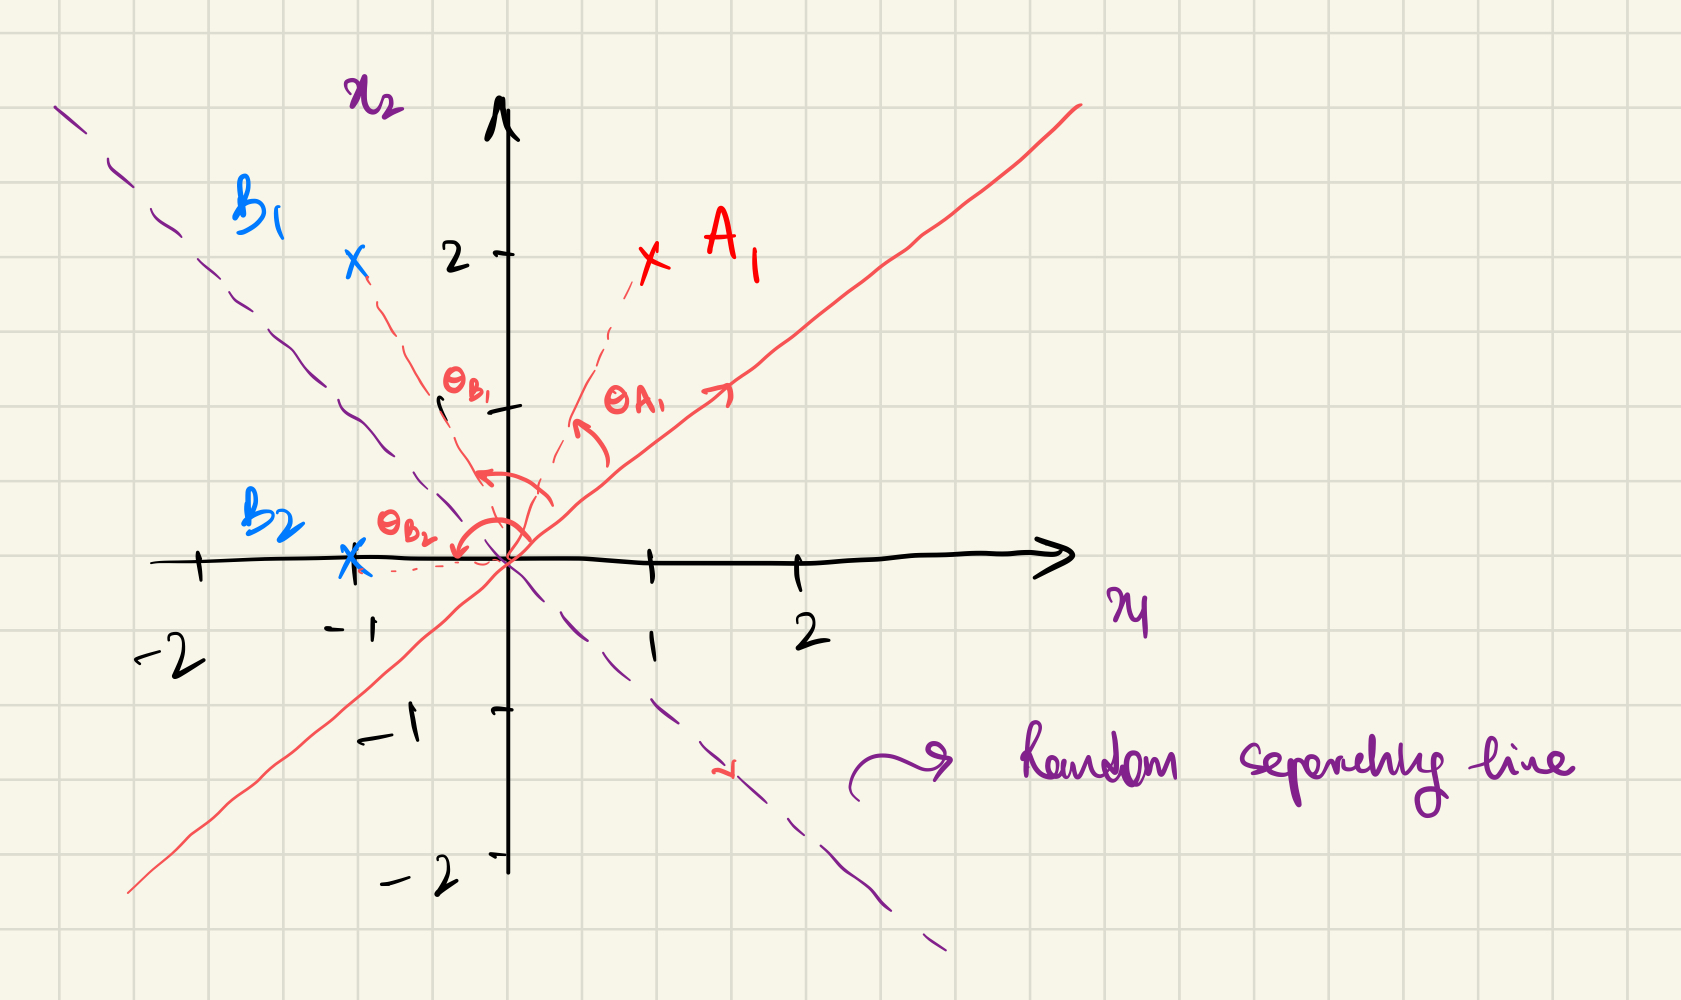
\includegraphics[scale=0.15]{CHAPTER_2/c2_fig_perceptron_example_3.jpeg}
  \caption{Caption}
  \label{fig:perceptron_example_3}
\end{figure}\\
Using the property of subtraction of vectors; we move the weight vector ($\textbf{w}$) away from $\textbf{B}_1$ and check the classification again. We  also introduce a learning rate $\alpha$ to control how much rotation we want. Let $\alpha = 0.5$
\begin{align}
  \textbf{w}^{(1)} &= \textbf{w} - \alpha\textbf{B}_1 \\
  &= \begin{bmatrix}
    1 \\
    1
  \end{bmatrix} - 0.5\begin{bmatrix}
    -1 \\
    2
  \end{bmatrix} \\
  & = \begin{bmatrix}
    1.5 \\
    0
  \end{bmatrix}
\end{align}\\
\begin{figure}[h]
  \centering
  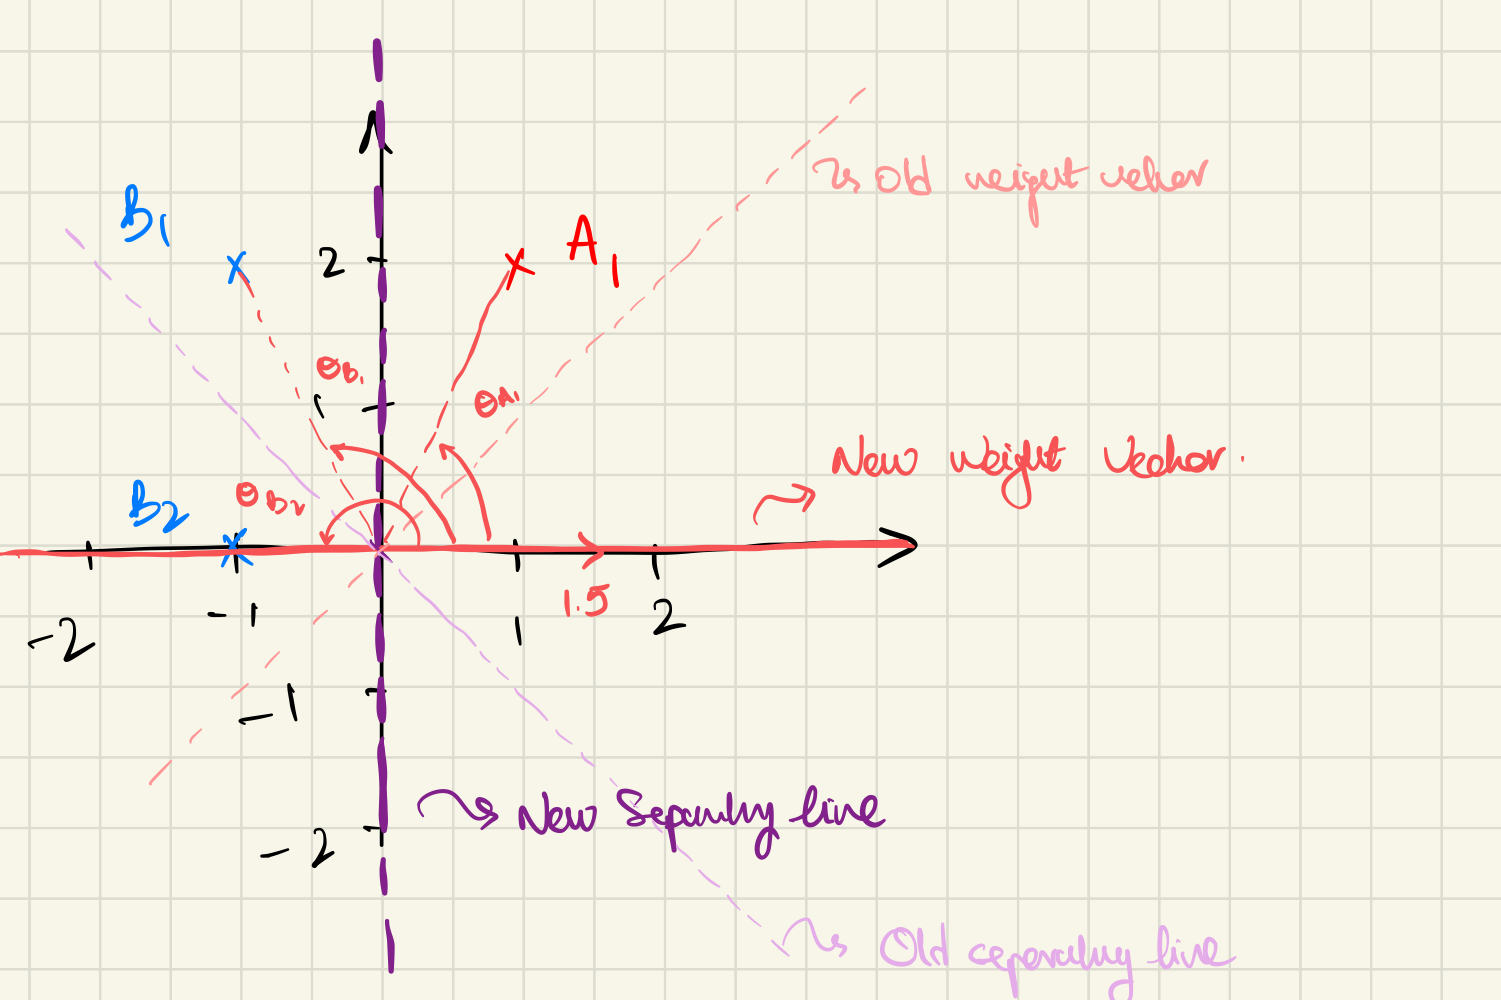
\includegraphics[scale=0.15]{CHAPTER_2/c2_fig_perceptron_example_4.jpeg}
  \caption{Caption}
  \label{fig:perceptron_example_4}
\end{figure} \\
Based on the new separating line, we can observe visually that the points are correctly classified. The computation of the binary classification using the new separating line $\textbf{w}^{(1)}$ is given by
\begin{align}
  f(A_1) &= f\begin{pmatrix}
    \begin{bmatrix}
      1.5\\
      0
    \end{bmatrix}.\begin{bmatrix}
      1 \\
      2
    \end{bmatrix}
  \end{pmatrix} = f(1.5) = 1 \\
  f(B_1) &= f\begin{pmatrix}
    \begin{bmatrix}
      1.5\\
      0
    \end{bmatrix}.\begin{bmatrix}
      -1 \\
      2
    \end{bmatrix}
  \end{pmatrix} = f(-1) = 0 \\
  f(B_2) &= f\begin{pmatrix}
    \begin{bmatrix}
      1.5\\
      0
    \end{bmatrix}.\begin{bmatrix}
      -1 \\
      0
    \end{bmatrix}
  \end{pmatrix} = f(-1.5) = 0
\end{align}
Thus, the perceptron learned how to classify the two sets of points. The function $f(\textbf{x})$ could be re-used to classify new points added to the sets.
\subsubsection{Perceptron Update Rule}
We can define a set number of rules for the perceptron to find the optimal weight vector to classify the points. Based on the properties of the dot product; the classification of the points are dependent on the inner angle between the normal of the separating line and the vector to be classified. If the inner angle is less than $90^\circ$ then the point belongs to class 1 else to class 0.\vspace{10mm}

\noindent \textbf{Target Classes and Errors} \\
Let the target(actual) classes be $y=1$ and $y=0$. Then the network error ${\epsilon}$ is given by the difference between the true value and the predicted value.
\begin{align*}
  \text{Network Error } \, \, \, \, \, \, \, {\epsilon}(\textbf{x}) &= y - f(\textbf{x})  \\
  \text{Correct Classification } \, \, \, \, y&=1, f(\textbf{x})=1 \rightarrow {\epsilon}(\textbf{x})=0 \\
  y&=0, f(\textbf{x})=0 \rightarrow {\epsilon}(\textbf{x})=0 \\
  \text{Incorrect Classification } \, \, \, \, y&=1, f(\textbf{x})=0 \rightarrow {\epsilon}(\textbf{x})=1 \\
  y&=0, f(\textbf{x})=1 \rightarrow {\epsilon}(\textbf{x})=-1
\end{align*}
We find that updating the weight vector can be written as
\begin{align}
  \textbf{w}^{(t+1)} = \textbf{w}^{(t)} + \alpha\epsilon(\textbf{x})\textbf{x}
\end{align}
\textbf{Perceptron Learning Algorithm}\\
The steps for the perceptron to learn how to perform binary classification is given by the steps below. Let $t$ be the $t^{th}$ iteration when learning and $b$ be in an input bias.

\vspace{5mm}
\noindent Assignment $\rightarrow$ Assign $t=0$, $\textbf{w}^{(0)} = (0,0,\dots,0)$, $b^{(0)}=0$\\
Start $\rightarrow$ For $t=0,1,2,\dots$ until convergence\\
\indent Step 1 $\rightarrow$ Randomly choose a vector $\textbf{x}^{(t)}$ with the corresponding $y^{(t)}$ (known)\\
\indent Step 2 $\rightarrow$ Compute $\textbf{z}=\textbf{w}^{(t)}.\textbf{x}^{(t)} + b^{(t)}$\\
\indent Step 3 $\rightarrow$ Compute $\epsilon^{(t)}(\textbf{z}) = y^{(t)} - f(\textbf{z}) $\\
\indent Step 4 $\rightarrow$ Update weight $\textbf{w}^{(t+1)} = \textbf{w}^{(t)} + \alpha\epsilon^{(t)}(\textbf{z})\textbf{x}^{(t)}$ \\
\indent Step 5 $\rightarrow$ Update bias  $b^{(t+1)} = b^{(t)} + \alpha\epsilon^{(t)}(\textbf{z})$
\vspace{10mm}
\\
The current perceptron we have defined is for a binary classification; we can also define multiclass perceptron and/or use different types of activation functions.
\subsubsection{Limitation of the Perceptron}
The perceptron alone is not always a good model to solve binary classification problem. It has certain limitation by nature of its definition. Consider the logic functions AND, OR and XOR across these 4 points:
\begin{align}
  \begin{matrix}
    \textbf{x}_1 = \begin{bmatrix}
      0 \\
      0
    \end{bmatrix},
    \textbf{x}_2 = \begin{bmatrix}
      1 \\
      0
    \end{bmatrix},
    \textbf{x}_3 = \begin{bmatrix}
      1 \\
      1
    \end{bmatrix},
    \textbf{x}_4 = \begin{bmatrix}
      0 \\
      1
    \end{bmatrix}  
  \end{matrix}
\end{align}
\subsubsection*{AND Function}
The AND function returns a value of 1 if both of the input is 1. 
\begin{align}
  \begin{matrix}
    f^{*}(\textbf{x}_1)=0,&   f^{*}(\textbf{x}_2)=0,&  f^{*}(\textbf{x}_3)=1,&   f^{*}(\textbf{x}_4)=0    
  \end{matrix}
\end{align}
\begin{figure}[h]
  \centering
  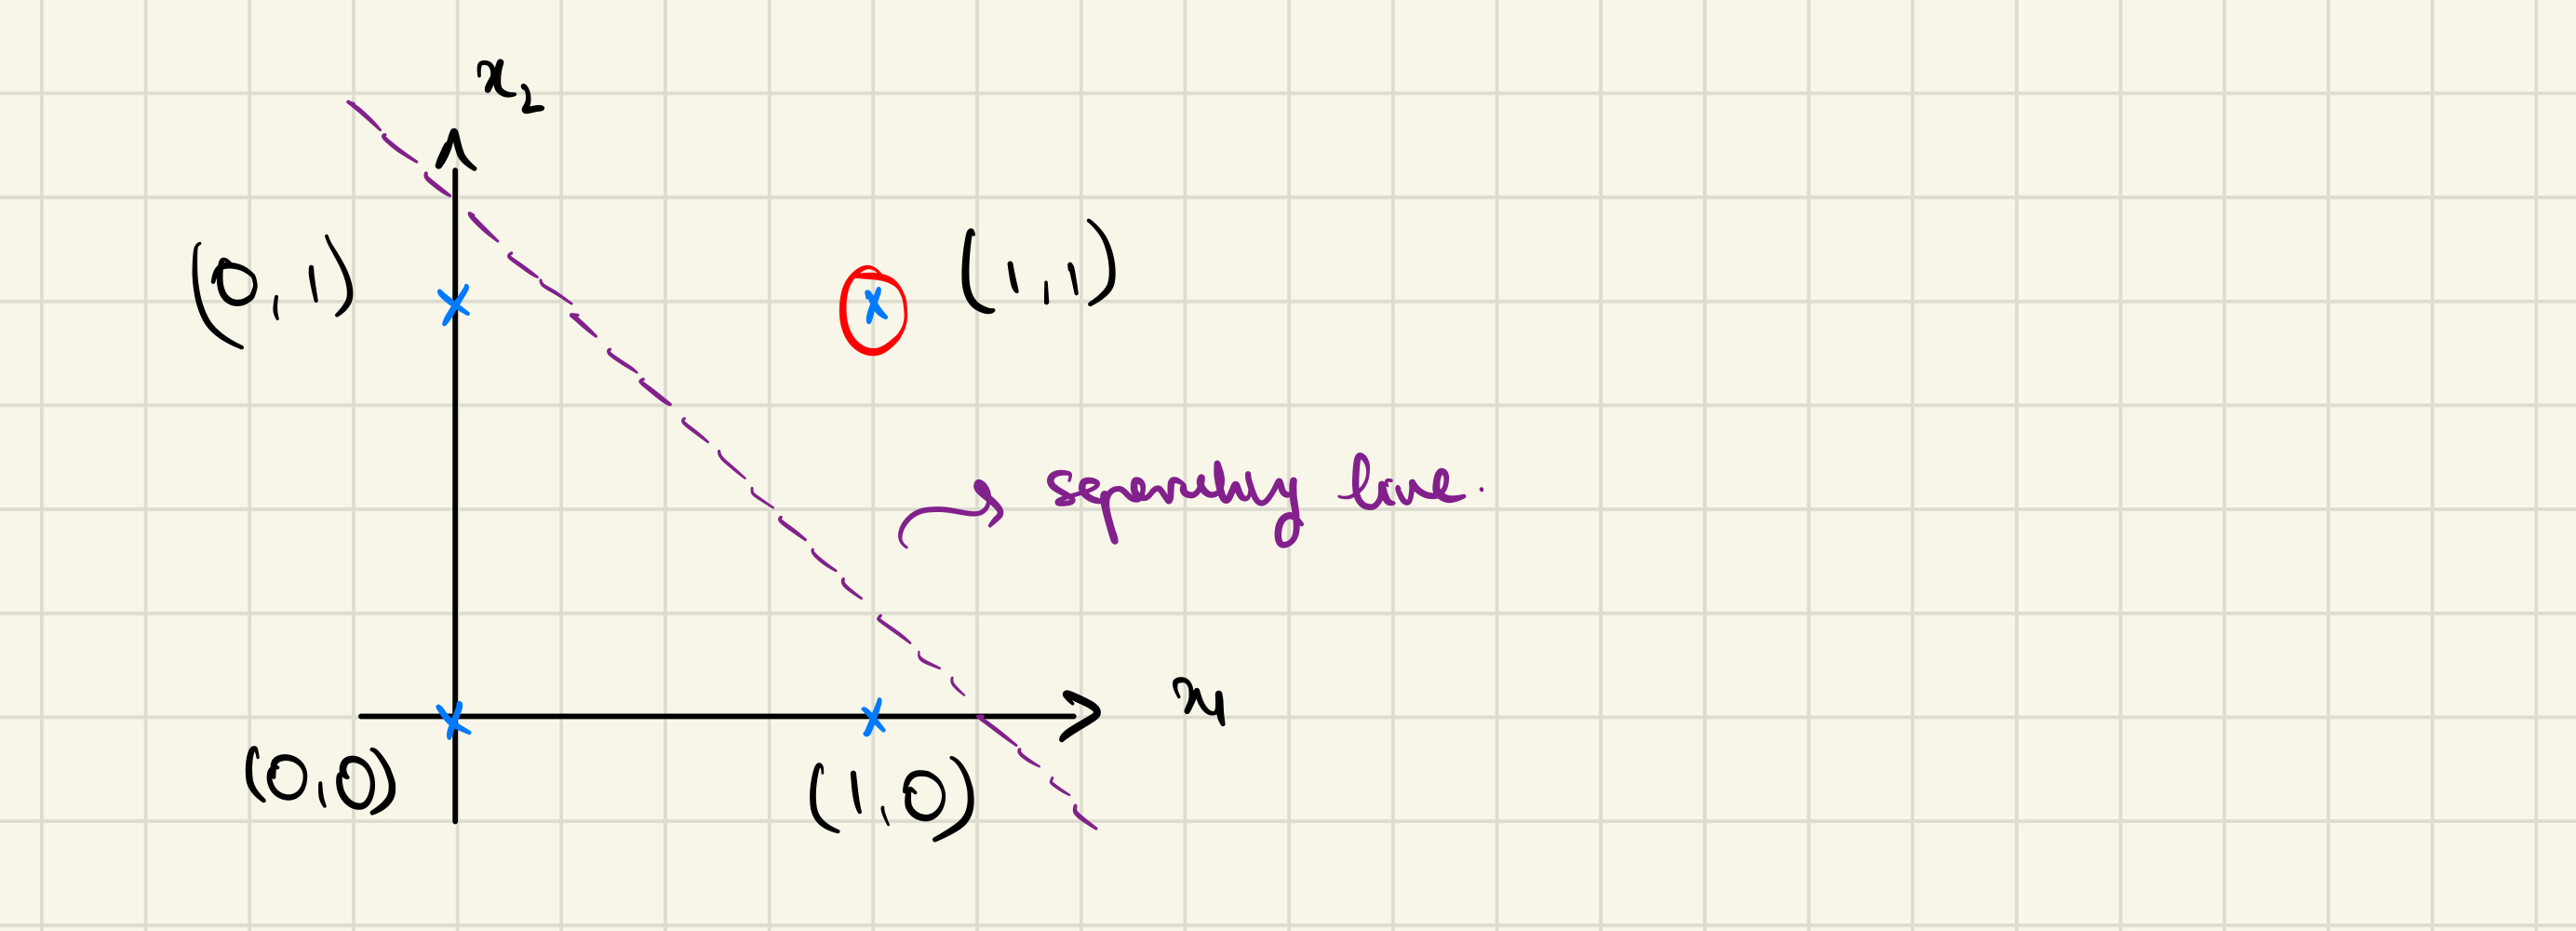
\includegraphics[scale=0.15]{CHAPTER_2/c2_fig_AND.jpeg}
  \caption{AND function}
  \label{AND_function}
\end{figure} \\
\noindent From figure \ref{AND_function}; we can easily define a separating line by the perceptron to separate the two classes.
\subsubsection*{OR Function}
The OR function returns a value of 1 if either of the inputs is 1.
\begin{align}
  \begin{matrix}
    f^{*}(\textbf{x}_1)=0,&   f^{*}(\textbf{x}_2)=1,& f^{*}(\textbf{x}_3)=1,&   f^{*}(\textbf{x}_4)=1    
  \end{matrix}
\end{align} \\
\begin{figure}[ht]
  \centering
  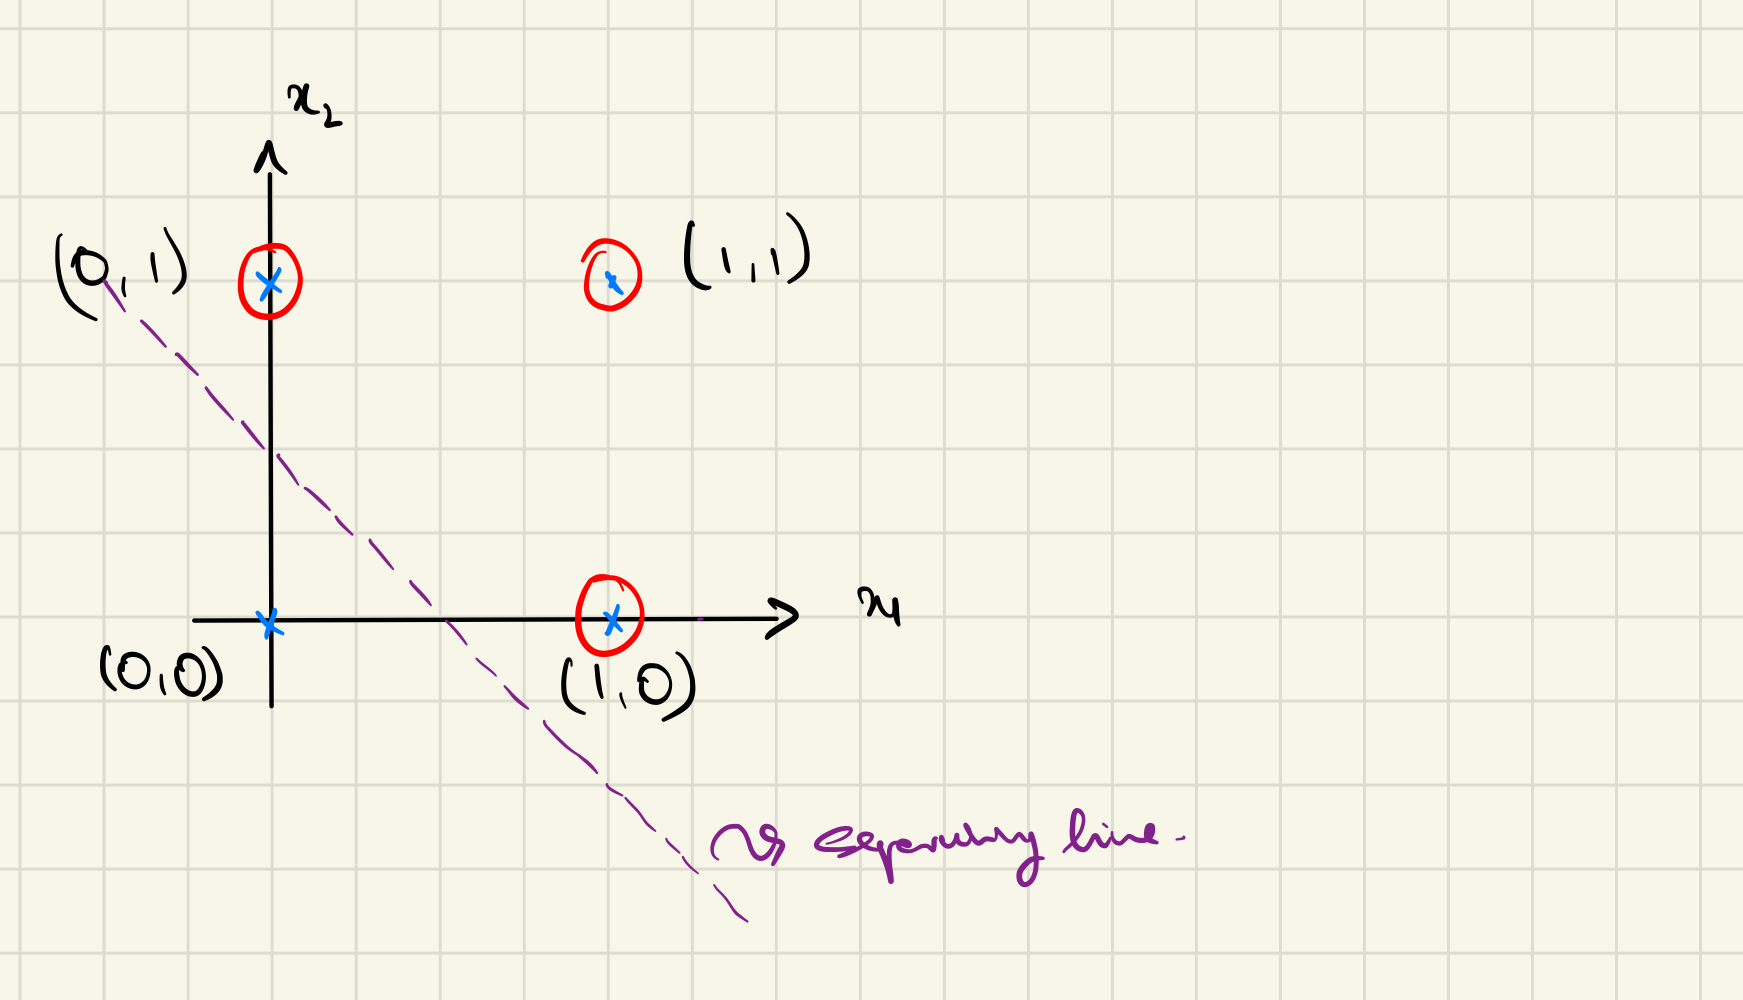
\includegraphics[scale=0.15]{CHAPTER_2/c2_fig_OR.jpeg}
  \caption{OR function}
  \label{OR_function}
\end{figure}
\vspace{100mm}
\noindent From figure \ref{OR_function}; we can easily define a separating line by the perceptron to separate the two classes.
\subsubsection*{XOR Function}
The XOR function returns a value of 1 if either of the inputs is 1 but not both.
\begin{align}
  \begin{matrix}
    f^{*}(\textbf{x}_1)=0,&   f^{*}(\textbf{x}_2)=1 ,& f^{*}(\textbf{x}_3)=0,&   f^{*}(\textbf{x}_4)=1    
  \end{matrix}
\end{align} 
\begin{figure}[h]
  \centering
  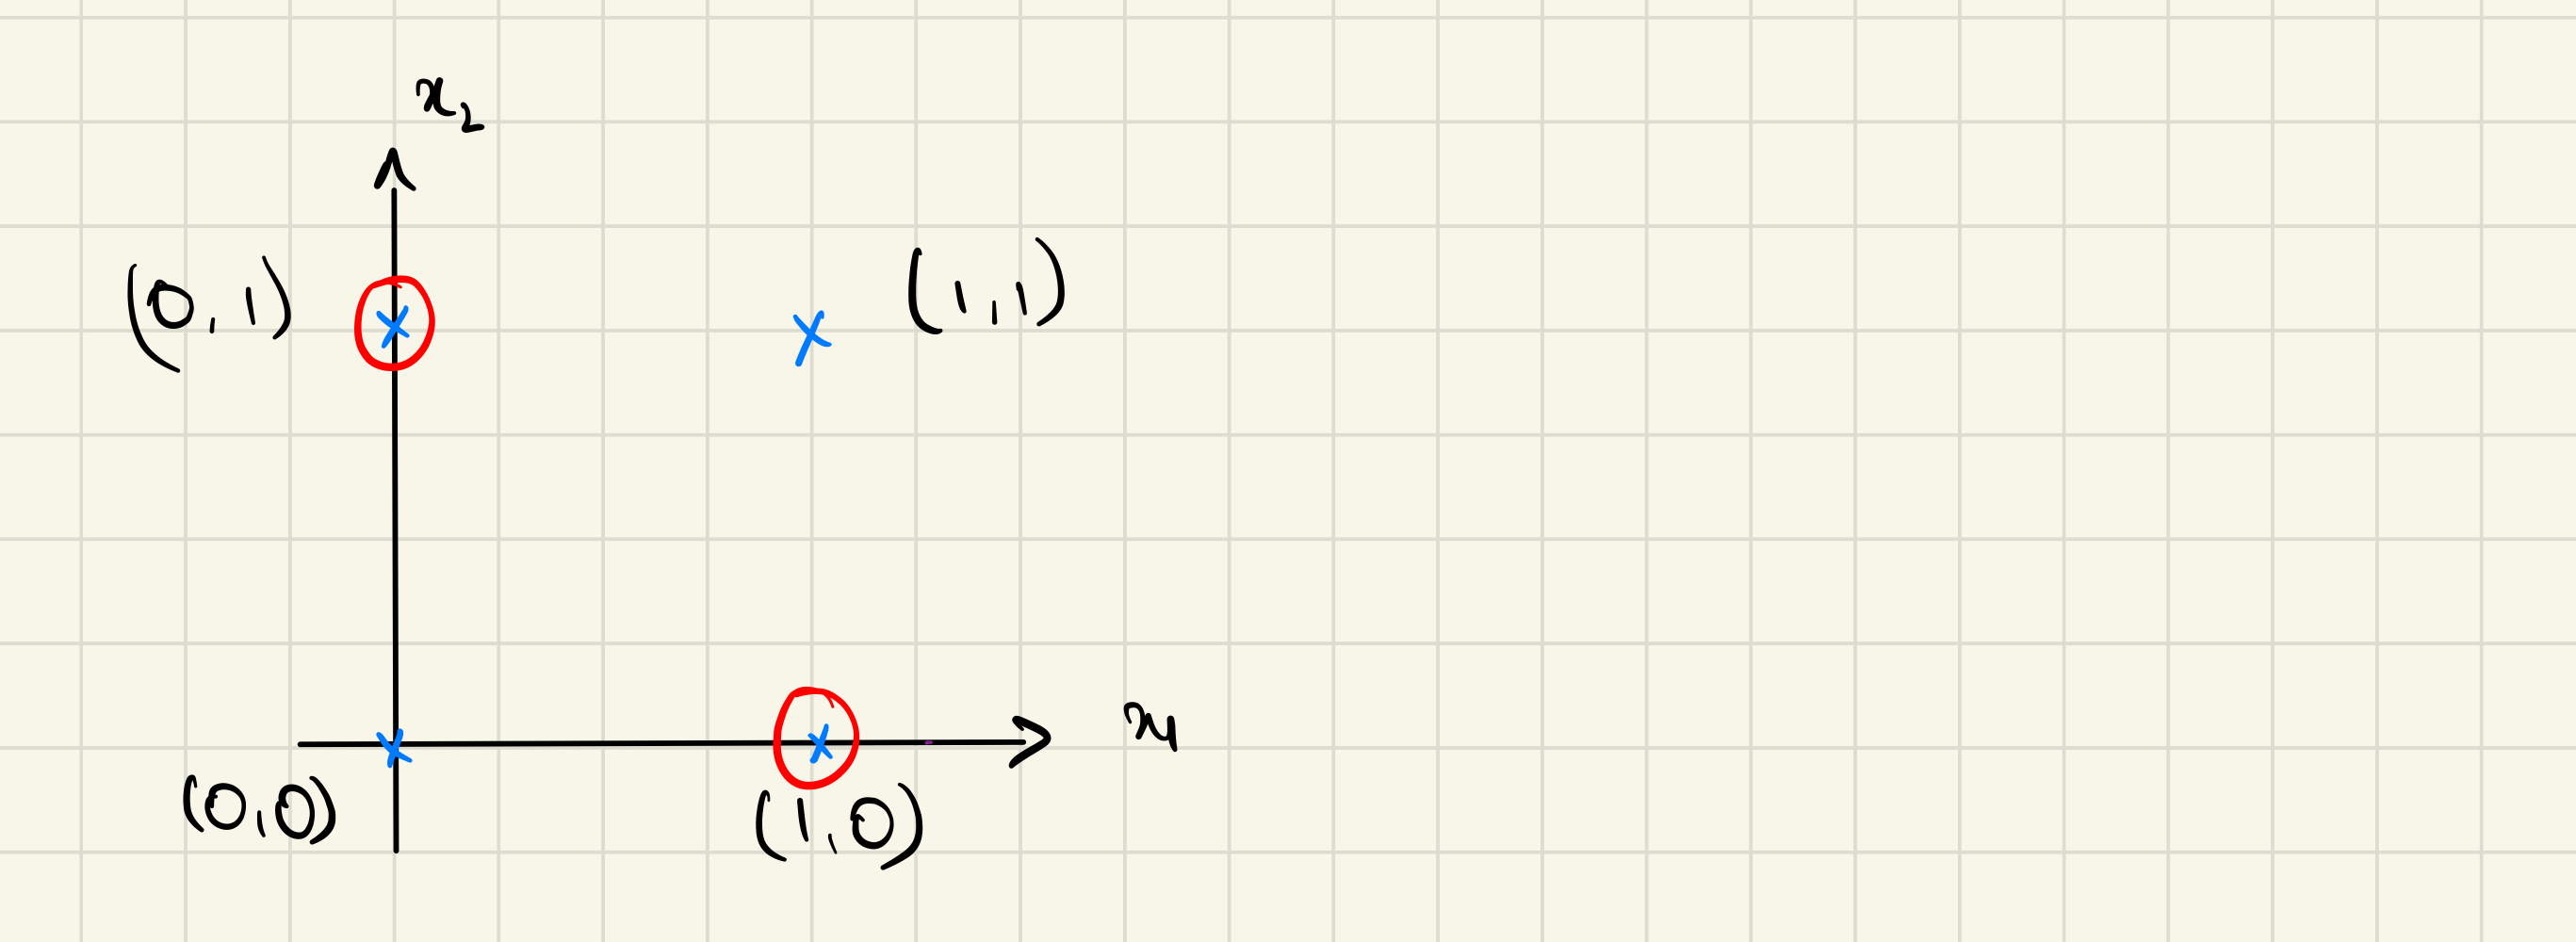
\includegraphics[scale=0.15]{CHAPTER_2/c2_rig_XOR.jpeg}
  \caption{OR function}
  \label{XOR_function}
\end{figure} \\
\noindent From figure \ref{XOR_function}; we can observe that no separating line alone could group the two different classes together. The perceptron model cannot solve the XOR logic function. Thus, we introduce \textbf{neural networks} to overcome this problem.
\subsection{Neural Network}
%- Combination of Neurons to form a network \refeq{fig:perceptron} - done
%- Feedfoward network - done
%- Explanation on how Network are just matrix multiplication - done
%- Explanation on error function and the generalization in Neural Network; and optimization problem - done
%- Adjusting the weight using Gradient Descent - done
%- Back propagation
A neural network is a set of perceptron connected together which takes an input, manipulate the information to learn from it and outputs a prediction. A neural network attempts to learn a mapping from an input to an output. The goal is to reduce the error between the prediction by the network compared to the true value as much as possible.
\begin{figure}[h]
  \centering
  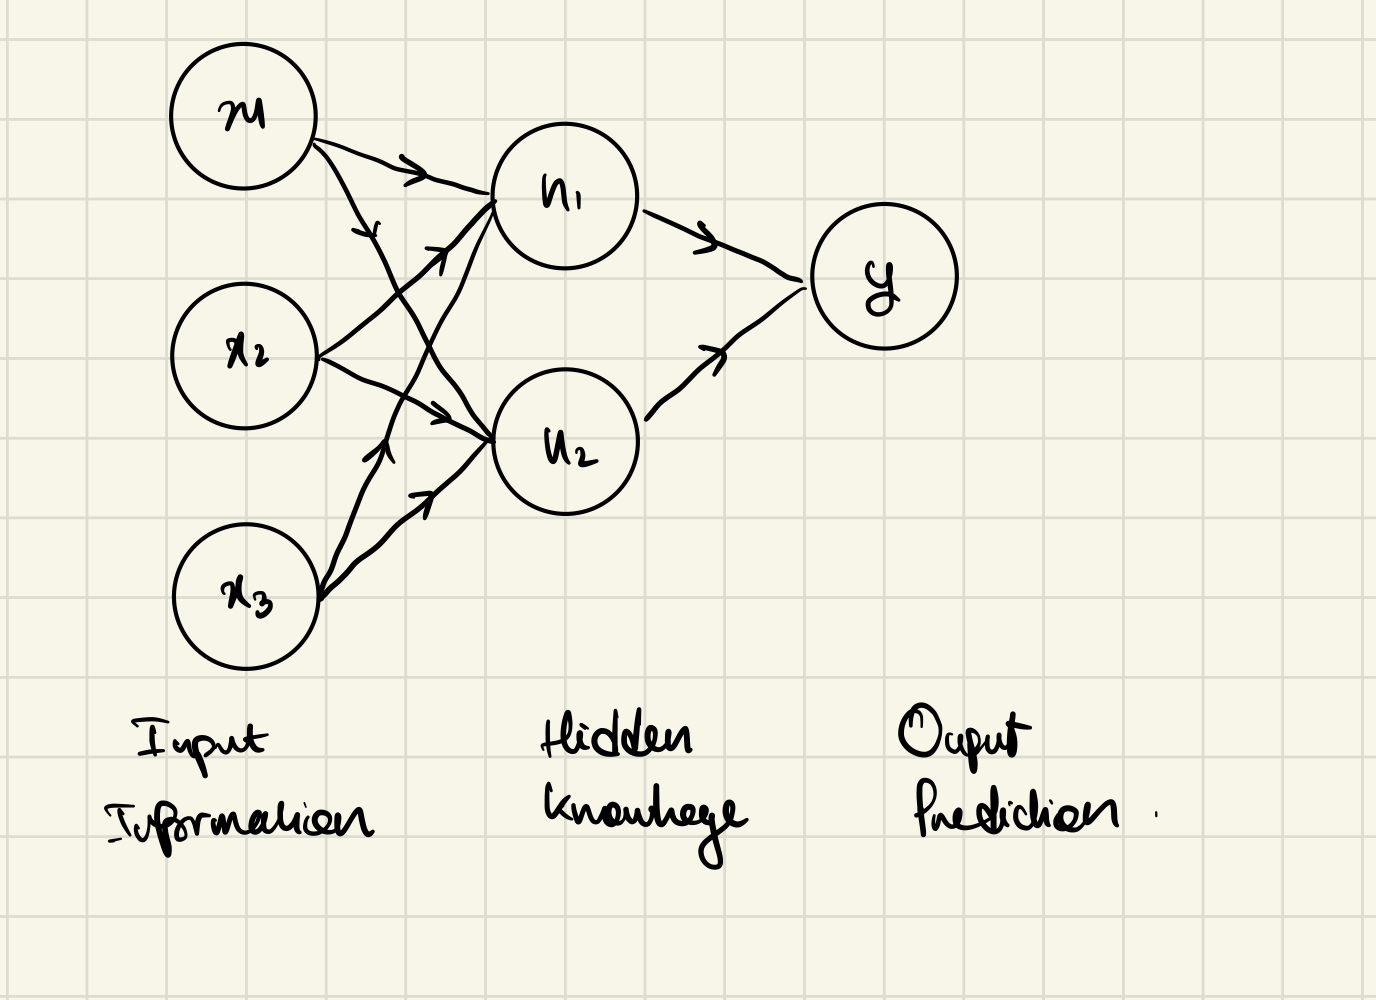
\includegraphics[scale=0.15]{CHAPTER_2/c2_fig_neural_network_1.jpeg}
  \caption{Caption}
  \label{neural_network}
\end{figure}
\vspace{10mm} \\
The neural network model can be represented by a series of matrix multiplication which takes the input and feeds the network. This is also known as a \textbf{feedforward network}.
\subsubsection{Feedforward Network}
Consider the simple network below with 2 input neurons, 2 perceptrons and 1 output.\\
\begin{figure}[!h]
  \centering
  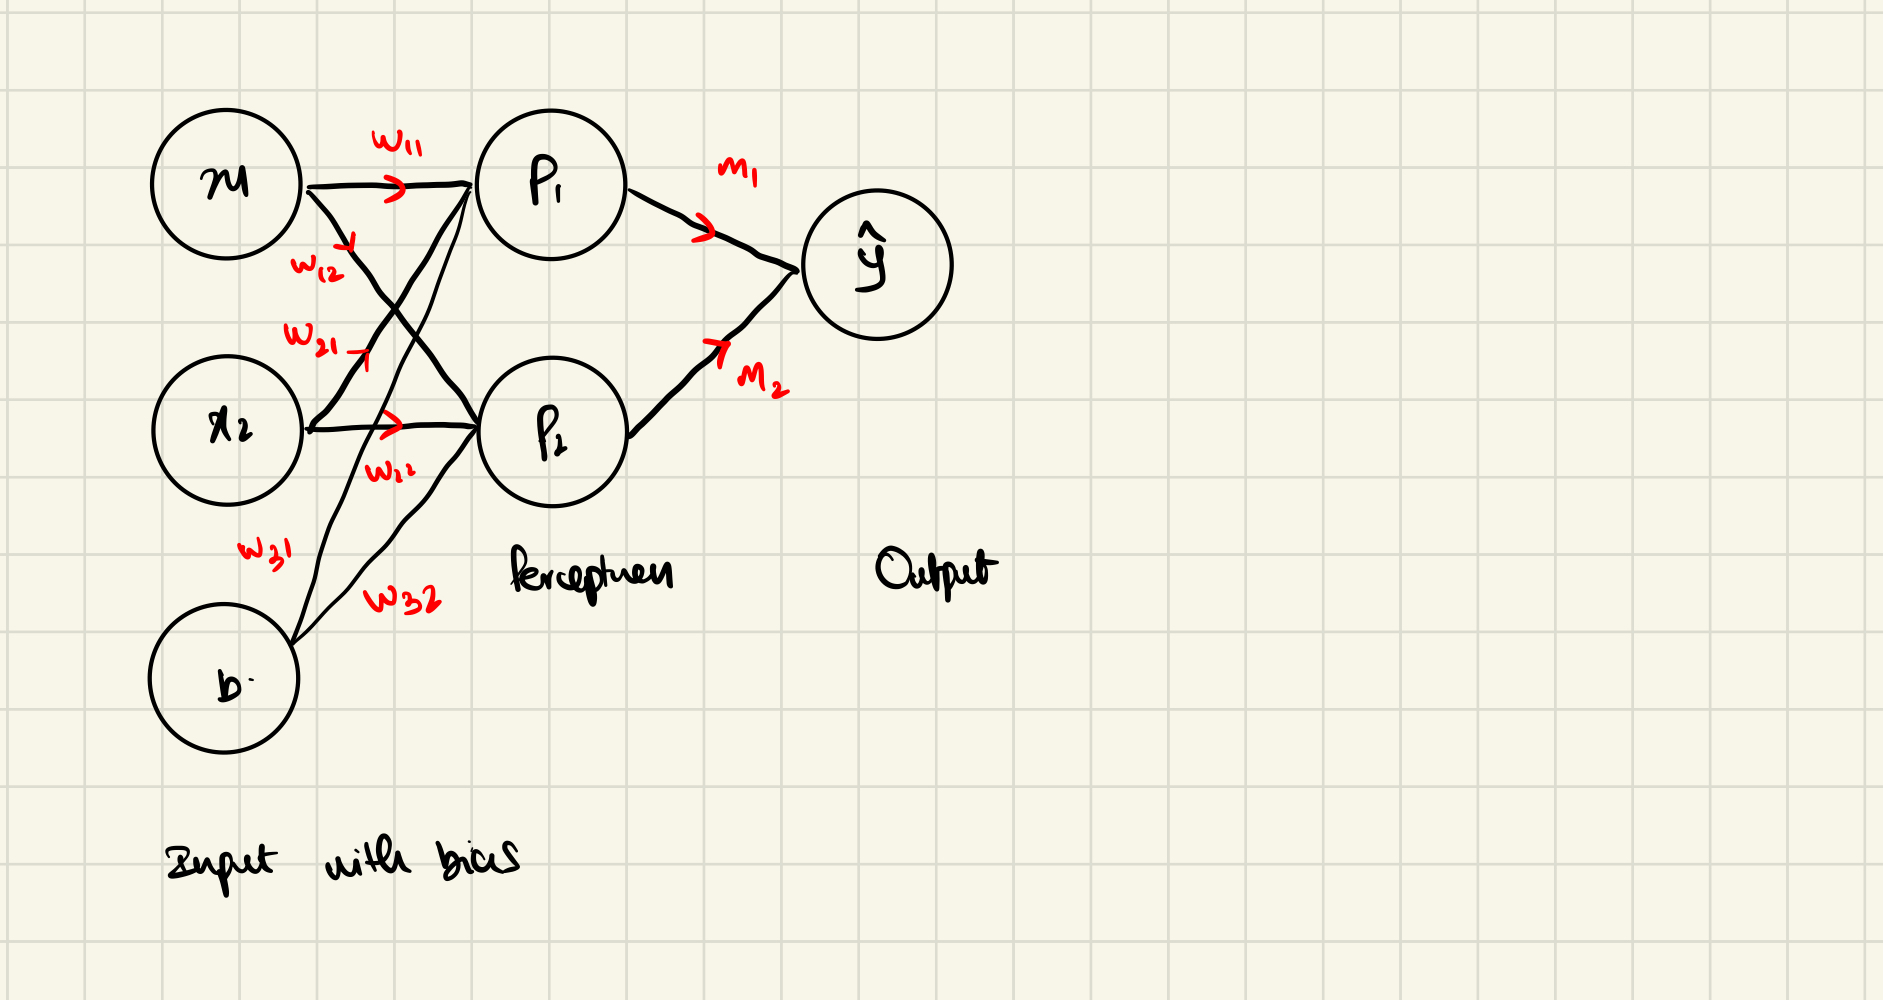
\includegraphics[scale=0.1]{CHAPTER_2/c2_fig_neural_network_2.jpeg}
  \caption{Caption}
  \label{neural_network_2}
\end{figure}
\vspace{20mm} \\
The feedforward network takes the information at the input and forwards it to the next layer after applying the weight vector for each respective hidden layer. This operation can be expressed as a series of matrix multiplication defined next. The input vector is given by $\textbf{x}$, random weight matrices by $\textbf{W}_i$ and the actual output be ${y}$.
\begin{align}
  \begin{matrix}
    \textbf{x} = \begin{bmatrix}
      x_{11} \\
      x_{21} \\
      b
    \end{bmatrix} & \textbf{W}_1 = \begin{bmatrix}
      w_{11} & w_{12} \\
      w_{21} & w_{22} \\
      w_{31} & w_{32}
    \end{bmatrix} & \textbf{W}_2 = \begin{bmatrix}
      m_{11} \\
      m_{21} 
    \end{bmatrix} &
    \textbf{y} = \begin{bmatrix}
      y
    \end{bmatrix}  
  \end{matrix}
\end{align}
The feedforward neural network for a single input vector can then be expressed as a series matrix multiplication to estimate the actual value of \textbf{y}. Let $\widehat{{y}}$ be the estimated value of ${y}$.
\begin{align}
  \widehat{{y}} &= f\begin{pmatrix}f(\textbf{x}^T\textbf{W}_1)\textbf{W}_2 \end{pmatrix} \nonumber\\
  &=f\begin{pmatrix}
    f\begin{pmatrix}\begin{bmatrix}
      x_{11} & x_{21} & b
    \end{bmatrix} \begin{bmatrix}
      w_{11} & w_{12} \\
      w_{21} & w_{22} \\
      w_{31} & w_{32} 
    \end{bmatrix}
  \end{pmatrix}\begin{bmatrix}
    m_{11} \\
    m_{21} 
  \end{bmatrix}
\end{pmatrix}
\label{neural_net_def}  
\end{align}
where $f$ is the function (\refeq{eq:perceptron_def}).
\subsubsection*{Solution to the XOR function}
One solution to the XOR function can be obtained using the neural network (\refeq{neural_net_def}) with the set go weights given by
\begin{align}
  \begin{matrix}
    \textbf{x} = \begin{bmatrix}
      x_{11} \\
      x_{21} \\
      -\frac{1}{2}
    \end{bmatrix} & \textbf{W}_1 = \begin{bmatrix}
      1 & -1 \\
      -1 & 1 \\
      1 & 1
    \end{bmatrix} & \textbf{W}_2 = \begin{bmatrix}
      1 \\
      1
    \end{bmatrix} &
    \textbf{y} = \begin{bmatrix}
      y
    \end{bmatrix}  
  \end{matrix}
\end{align}
\textbf{Verifying the Solution}
\begin{align}
  \begin{matrix}
    \begin{bmatrix}
      x_{11} \\
      x_{12}
    \end{bmatrix} = \begin{bmatrix}
      0 \\
      0
    \end{bmatrix} \rightarrow & \widehat{y} = 0 & 
    \begin{bmatrix}
      x_{11} \\
      x_{12}
    \end{bmatrix} = \begin{bmatrix}
      1 \\
      0
    \end{bmatrix} \rightarrow & \widehat{y} = 1 \\
    \\
    \begin{bmatrix}
      x_{11} \\
      x_{12}
    \end{bmatrix} = \begin{bmatrix}
      0 \\
      1
    \end{bmatrix} \rightarrow & \widehat{y} = 1 & 
    \begin{bmatrix}
      x_{11} \\
      x_{12}
    \end{bmatrix} = \begin{bmatrix}
      1 \\
      1
    \end{bmatrix} \rightarrow & \widehat{y} = 0
  \end{matrix}
\end{align}
The neural network correctly classifies all input. While feed-forward network of this form helped us to solve the XOR function it is very limited. The architecture defined can only be used for linearly separable problem. In order to allow for non-linear solution; we need to introduce some non-linearity in the model. This is done by using different kinds of \textbf{activation functions} in the perceptrons.
\subsubsection{Activation Functions}
Activation functions can be used with a perceptron to introduce non-linearity. The function to be used is subjective to the problem being solved and the form of the desired result we want. Some activation functions are defined below.\\
\textbf{Linear}
\begin{align}
  \phi(z) = z
\end{align}
\textbf{Unit Step (Heaviside Function)}
\begin{align}
  \phi(z) = \begin{cases}
    0 & z<0 \\
    0.5 & z=0 \\
    1 & z>0
  \end{cases}
\end{align}
\textbf{Signum}
\begin{align}
  \phi(z) = \begin{cases}
    -1 & z<0 \\
    0 & z=0 \\
    1 & z>0
  \end{cases}
\end{align}
\textbf{Sigmoid}
\begin{align}
  \phi(z) = \frac{1}{1+ e^{-z}}
\end{align}
\textbf{Hyperbolic Tangent(tanh)}
\begin{align}
  \phi(z) = \frac{e^z - e^{-z}}{e^z + e^{-z}}
\end{align}
\textbf{ReLU}
\begin{align}
  \phi(z) = \begin{cases}
    0 & z<0 \\
    z & z>0
  \end{cases}
\end{align}
\subsubsection{Network Error}
The network error is given by the squared difference between the predicted value and the true value. The difference is squared to avoid the sum of errors of multiple input vector to be zero which can mislead the network to have perfect predictive power.
\begin{align}
  \text{Network Error } e = \dfrac{1}{2}\sum^{\text{Total Input}}_i (\widehat{y_i}-y_i)^2
  \label{network_error}
\end{align}
The goal of the network is to adjust the weight to reduce the network error as much as possible. The idea of reducing a function to a value is synonymous to (\refeq{eq:optimization_problem}) an optimization problem. The network error in (\refeq{network_error}) is a quadratic equation.\\
\begin{figure}[ht]
  \centering
  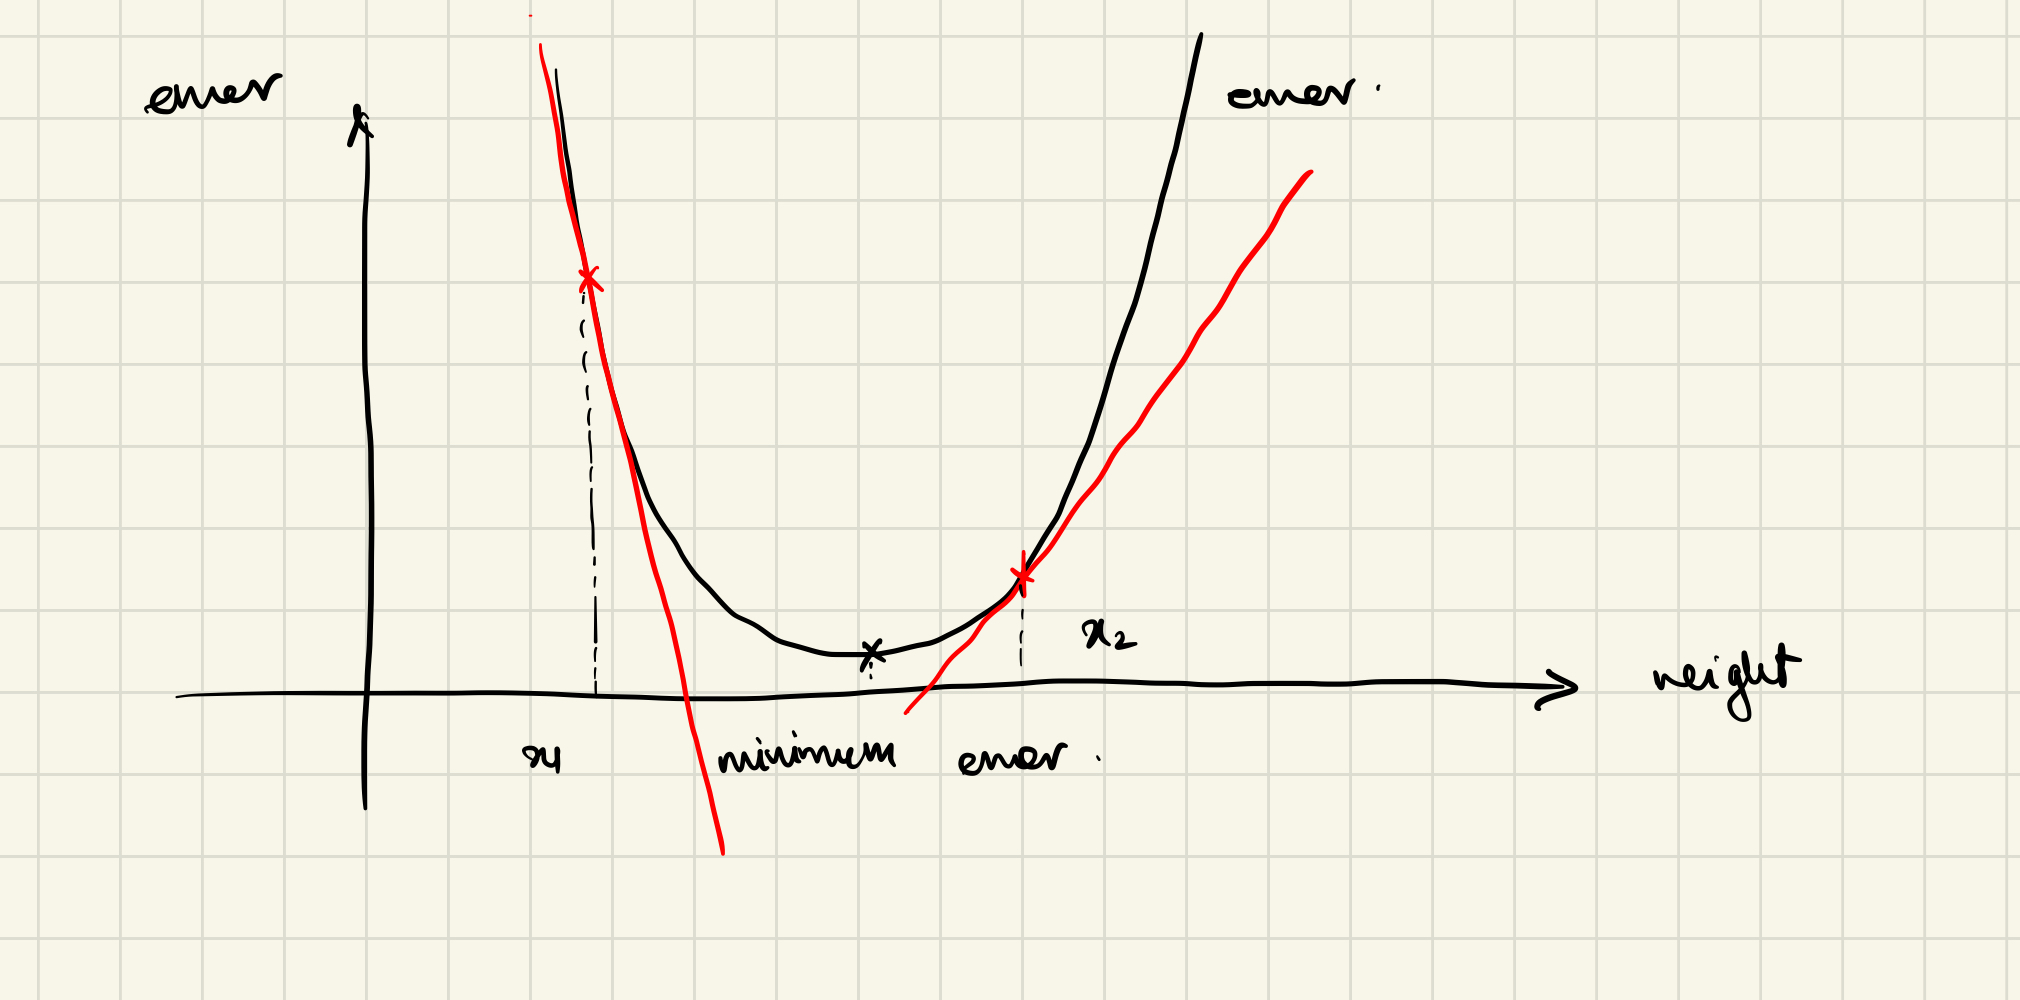
\includegraphics[scale=0.15]{CHAPTER_2/c2_fig_network_error.jpeg}
  \caption{Network Error}
  \label{network_error_graph}
\end{figure}\vspace{70mm}\\
Figure (\ref*{network_error_graph}) is a graphical representation of the network error function. Our goal is to reach the minimum of the function by adjusting the weight value. We use the \textbf{gradient descent method} to reach the bottom of the curve.
\subsubsection{Gradient Descent Method}
In order to reach the bottom of the function; we need to adjust the weight such that the derivative of the error function is 0. The approach of updating the weight based on the gradient of the error function is known as \textbf{gradient descent}. The derivative with respect to the weights of the network error (\refeq{network_error}) for a single input is given by
\begin{align}
  \frac{de}{dw_{ij}} = (\widehat{y_i}-y_i)\frac{d\widehat{y_i}}{dw_{ij}}
  \label{derivative_network_error}
\end{align}
From figure (\refeq{network_error_graph}); we can observe that if the gradient is negative then we have underestimated the predicted value and need to increase the weight to reach the optimal value. On the other hand, if the gradient is positive then we have overestimated the predicted value and need to decrease the weight to reach the optimal value. The equation (\refeq{derivative_network_error}) provides us with the opposite direction and amount to adjust the weight. Hence, the update rule of the weights for gradient descent method is given by
\begin{align}
  w_{ij}^{t+1} = w_{ij}^{t} - \dfrac{de}{dw_{ij}}
\end{align}
In the gradient descent method, the network learns from the gradient of the error function and adjust the weights accordingly to reduce the error. However, the gradient alone can be quite large, causing oscillations as we go down the error function. We fix this problem by introducing a \textbf{learning rate} $\alpha$ prior to adjusting the weight.
\subsubsection{Learning Rate}
The learning rate is typically denoted by the Greek letter alpha $\alpha$. It helps the network to control the rate at which the weights are changing. Having a system with a high learning rate may lead to an oscillating network when trying to find the optimal weight and having a slow learning rate increases the number of iterations required when optimizing the network. The adjusted update rule of the weight is given by
\begin{align}
  w_{ij}^{t+1} = w_{ij}^{t} - \alpha\dfrac{de}{dw_{ij}}
\end{align}
where $\alpha \in (0,1)$
\subsubsection{Back Propagation}
The input data has been fed forward in the network. Then the error function and the gradient descent method we have defined are both executed at the end of neural network we have defined in equation (\refeq{neural_net_def}). We now need a way to back propagate the weight changes that need to happened from the output neuron to the input neuron. This whole process is known as \textbf{back propagation}.
\subsection{Deep Neural Network}
%- Explain why Deep Neural Network multiple-layer backpropagation
%- Different types of activation function
%- Back propagation in deep neural network explanation
\subsection{Overfitting}
\subsubsection{Dropout}
\subsection{Convolutional Layer}